\section{Machine Learning}
\label{sec:ml-primer}

\noindent We begin by presenting the main ingredients in the machine learning pipeline:
%
\begin{itemize}
    \item a dataset $\mathcal{D}$, made out of
          \textit{inputs} $\mathcal{D}=\left\{\bm{x}_n\right\}_{n=1}^N$ or
          \textit{input-output} pairs
          $\mathcal{D}=\left\{(\bm{x}_n,y_n)\right\}_{n=1}^N$;
    \item a set of parameters $\theta$;
    \item a loss function $L$.
\end{itemize}
%
With these ingredients, we create a machine learning pipeline by
taking a \textit{training set} that is a subset of $\mathcal{D}$ and estimate
the parameters $\theta$ by minimizing the loss
$L$ on that set. The resulting model with optimal
$\hat{\theta}$ can then be evaluated on a held-out set of
$\mathcal{D}$, called \textit{test set}, to assess its performance.
We will often assume $\mathcal D$ is made out of input-output pairs,
unless specified otherwise.

When the model is probabilistic, this process creates a probability
model that identifies the probability measure of a random experiment:
it maps from available inputs in the set of possible inputs
$\mathcal{X}$ to a probability distribution of a random variable $Y$. When the set of
possible outputs $\mathcal{Y}$ is discrete, the probability
distribution of $Y$ is prescribed by a probability mass function
(pmf) $p_{Y|X}(y|\bm{x};\theta)$; when the set of possible outputs
$\mathcal{Y}$ is continuous, the probability distribution of $Y$ is
prescribed by a probability density function (pdf). In the context of
the present thesis, we will not have applications in which
$\mathcal{Y}\in\reals$ (\ie, \textit{regression problems}) and as
such, when referring to $p_{Y|X}(y|\bm{x};\theta)$, we assume that it is a
probability mass function. Furthermore, our problems will most often
involve a $k$-way classification, and so $p_{Y|X}(y|\bm{x};\theta)$ will be
specifying a \textit{Categorical} distribution,
%
\begin{equation}
    Y|X\!\!=\!\bm{x}~\sim \text{Cat}(f(\bm{x}; \theta)),
\end{equation}
%
where $f(x; \theta) \in \simplex^{K-1}$ is a function such that
$p_{Y|X}(y|\bm{x};\theta)=\text{Cat}(y|f(\bm{x}; \theta))$.

\paragraph*{Supervised learning.} We now turn our attention to applications
in which one uses a dataset of input-output pairs. In such a case,
to estimate $\theta$ we minimize the loss over the input-pair dataset,
%
\begin{equation}
    \hat{\theta} = \argmin_\theta L_\mathcal{D}(\theta),
\end{equation}
%
where $L_\mathcal{D}(\theta)$ is the loss function:
the \textit{negative log-likelihood}
%
\begin{equation}
    L_\mathcal{D}(\theta) = -\mathcal{L}_\mathcal{D}(\theta) =
    - \sum_n \log p_{Y|X}(y_n|\bm{x}_n; \theta).
    \label{eq:discr-loss}
\end{equation}
%
A model with the loss function of \eqnref{eq:discr-loss} is called a
\textit{discriminative model}, while one that models instead
$p_{XY}(\bm{x}, y; \theta)$ is called a \textit{generative model}.
Typically, the loss function might also entail a regularization term (\eg, the $\ell_2$ norm),
which is added to the negative log-likelihood
%
\begin{equation}
    L_\mathcal{D}(\theta) = -\mathcal{L}_\mathcal{D}(\theta) + \mathcal{R}(\theta).
\end{equation}
%
Sometimes, instead of the probabilistically-grounded negative
log-likelihood, practitioners might use a non-probabilistic loss $\ell$ and
still use a statistical model; for example, one might use the 0/1
loss where the loss is $1$ if the $\argmax$ mode is wrong (\ie,
$\hat{y}\neq y$) and $0$ otherwise. After training the model, we wish
to make predictions $\hat{y}$ for each novel input $\bm{x}$ of the
test set, and we can make such predictions by using the optimal
trained parameters $\hat{\theta}$ and selecting, for instance, the highest-scoring
$y\in\mathcal{Y}$ by taking the $\argmax$
%
\begin{equation}
    \hat{y}=\argmax_{y\in\mathcal{Y}}p_{Y|X}\left(y|\bm{x};\hat{\theta}\right).
\end{equation}
%
For example, in a binary sentiment classification problem of English
sentences, $\mathcal{Y}=\{\text{negative},\text{positive}\}$, and
$\mathcal{X}$ would be the set of possible sentences in the English
language.

\paragraph*{Unsupervised learning.} Similarly, there are also applications in machine learning where we use just a
dataset of inputs $\mathcal D = \left\{\bm{x}\right\}_{n=1}^N$ and estimate the parameters $\theta$ under a loss to
obtain an unsupervised model; that is, a model in which inferences are made
without access to any labels (\ie, outputs). In this case, the loss function $L$ only
depends on the inputs $\bm{x}_n$ and the parameters $\theta$
and we thus model $p_X(\bm{x}|\theta)$.
In this case, the loss function is
%
\begin{equation}
    L_\mathcal{D}\left(\theta\right)=-\sum_n\log p_X\left(\bm{x}_n|\theta\right).
\end{equation}
%
In this setting, to assess the resulting model's performance,
we often compute the log-likelihood of the model under the test set
%
\begin{equation}
    \mathcal{L}_{\mathcal{D}_\text{test}}(\hat{\theta}) =
    \sum_n\log p_X\left(\bm{x}_n|\hat{\theta}\right),
\end{equation}
%
that is, we assess the likelihood of the model being able to generate
the data points $\bm{x}$.

\paragraph*{Semi-supervised and weakly-supervised learning.} In a
semi-supervised setting, there is typically a smaller portion of the
dataset that is labeled,
$\mathcal{D}_{L}=
    \left\{(\bm{x}_n,y_n)\right\}_{n=1}^{N_{L}}$,
and the remaining majority is unlabeled,
$\mathcal{D}_{U}=
    \left\{(\bm{x}_n)\right\}_{n=1}^{N_{U}}$.
The parameters are then estimated by using a combination of losses: a
component that is supervised and another that is unsupervised.
Taking the loss examples given above, a probabilistic semi-supervised model could
have the loss function
%
\begin{equation}
    L_{\mathcal D}\left(\theta\right)=
    -\sum_{\bm{x}\in\mathcal{D}_U}
    \log p_{X}\left(\bm{x}|\theta\right)
    -\sum_{(\bm{x},y)\in\mathcal{D}_L}
    \log p_{XY}\left(\bm{x}, y;\theta\right).
    \label{eq:semisup}
\end{equation}
%
In some applications,
both models may be independent components that share some
parameters; in others, they are components of the same joint distribution over
$\mathcal{X}\times\mathcal{Y}$.
In the context of this
thesis, we will use the term \textit{weakly-supervised} and
\textit{weak supervision} to refer to a broader setting that aims to
alleviate the need for labeled data to obtain a well-performing
model. This setting not only includes semi-supervision but also
includes, for example, the transferring of learned parameters of an
already optimized unsupervised model to a supervised one, also called
\textit{transfer learning}. In such a case, the estimation of
parameters can first occur by minimizing the first loss component in
\eqnref{eq:semisup}, and then those learned parameters can be reused
as an initialization on the minimization of the second component.
While not explored in this thesis, other forms of weak supervision
include the usage of underspecified or unreliable labels, linguistic
constraints, labels obtained via heuristics, among others.

\subsection{Linear and Deep Models}

\noindent Naturally, there are many different ways one can use $\theta$ to
parameterize $p_{Y|X}\left(y|\bm{x};\theta\right)$. One of the simpler ways
is to define a log-linear model
%
\begin{align}
    p_{Y|X}\left(y|\bm{x};\theta\right) & = \text{Cat}(y|f(\bm x; \theta)) \\
    f(x; \theta)                        & = \softmax \left(\bm{s}\right)   \\
    \bm{s}                              & 
    = \bm{W}_{\theta}^T\bm{\phi}\left(\bm{x}\right) \label{eq:linear}
\end{align}
%
where $\bm{\phi}$ is a function that maps $\bm{x}$ into a
manageable space, $W_{\theta}$ is a matrix of learnable weights, and
\textbf{softmax} is a function that maps a vector of scores $\bm{s}\in\reals^K$ into
a ``vector of probabilities'', that is, $\sum_{k=1}^K\left[\softmax(\bm{s})\right]_k=1$
and $\left[\softmax(\bm{s})\right]_k \geq 0$.

\begin{definition}[softmax]
    The mapping function \textbf{softmax} is defined as
    \begin{equation}\label{eq:softmax}
        \left[\softmax(\bm{s})\right]_j = \frac{\exp(s_j)}{\sum_{j'} \exp(s_{j'})}.
    \end{equation}
\end{definition}

In these linear models, the problem of obtaining the optimal $\bm{W}_{\theta}$ lies
within the set of problems that convex optimization can solve, which
significantly simplifies the optimization process. While the
optimization simplicity of linear models is appealing, constructing a suitable
$\bm{\phi}$ may require significant effort. The creation of an
effective feature function $\bm{\phi}: \mathcal{X} \rightarrow \reals^d$ might
demand extensive knowledge of the domain of $\mathcal{X}$ and of the
task itself. The \textit{art} of creating these functions $\bm{\phi}$
is often called \textbf{feature engineering}.

An alternative to the log-linear model is a \textbf{neural network}, which, in a
way, performs feature engineering automatically through the use of hidden
representations. Neural networks use non-linear functions, also known
as \textit{activation functions}, along with linear functions similar
to \eqnref{eq:linear} in order to build these hidden representations.

\begin{definition}[neural network]
    A neural network with parameters $\theta$ is a function
    composed of building blocks that comprise both linear and non-linear
    functions. These building blocks are called \textit{layers}.
    The layers connect in a sequence, and the output of each
    layer is fed into the next layer. The output of the last layer is
    the output of the neural network
    %
    \begin{equation}
        f(x; \theta) = \pi 
        \left(\bm{W}_{\theta}^T\bm{\phi}_{\theta}\left(\bm{x}\right)\right)\,,
    \end{equation}
    %
    where compositions of differentiable functions with learnable
    $\theta$ parameterize $\bm{\phi}_{\theta}$ and $\pi$ is a
    function that projects the scores into vectors of probabilities (\eg, softmax).
    The composition of $\bm{\phi}_{\theta}$ is extremely flexible and
    can be defined in a variety of ways, making it a powerful way to
    obtain meaningful representations of the input space.
\end{definition}
%
Thanks to its non-linearities, neural networks effectively create
intermediate abstractions of the data, which are optimized to represent the data
more effectively in order to succeed at the task, bypassing the need
for feature engineering.

Just as well, non-linearities and the flexible composition of functions end up
impeding the usage of convex optimization, and so neural networks are
often trained instead through a process called
\textit{backpropagation}, a gradient-based optimization algorithm.

\begin{definition}[backpropagation]
    Backpropagation is a gradient-based optimization algorithm that
    locally minimizes the loss function $L$ by iteratively updating the
    parameters $\theta$. In order to be able to update $\theta$,
    the only requirement is to be able to compute the gradient of
    $L$ with respect to every coordinate $\theta_d\in\theta$:
    %
    \begin{equation}
        \frac{\partial L_{\mathcal{D}}(\theta)}{\partial \theta_d}.
        \label{eq:backprop}
    \end{equation}
    %
\end{definition}

Due to the simplicity of this requirement, practitioners can build
neural networks in a modular way, where differentiable building
blocks of functions are combined in arbitrary computational graphs. A
handful of different algorithms can be used to update $\theta$ during
backpropagation; for example, Adam~\citep{kingma2014adam}.

In practice, computing \eqnref{eq:backprop} for the whole dataset
$\mathcal D$ is a costly operation, and so the gradient is usually
computed through an unbiased estimate: independent and identically
distributed samples of the dataset are drawn at each iteration, and \eqnref{eq:backprop}
is computed on that set of samples (\ie, the \textit{mini-batch}).
The size of the step at which $\theta$ is updated is determined by a value usually called the learning rate,
which is a hyperparameter of the model that is chosen to maximize a given metric on a held-out
dataset (the \textit{validation set} or \textit{development set}).

\section{Neural Networks and Natural Language}

\noindent Using neural networks in NLP applications is a pivotal part
of the research shown in the present thesis. While there are many
ways of applying neural networks to NLP, exploiting many different
architectures and aimed at many different tasks, we give
special attention to sequence-to-sequence models, which we will
explain in the sequel.

Nevertheless, in the context of neural networks for NLP, there is a
clear focus on obtaining vectorized representations of words, of words
within their context, and of whole sentences. A common ingredient in all
neural network architectures of NLP is the use of
\textbf{embeddings}. After the sentence is segmented into tokens
(words, segments of words, and punctuation), the first component of the
neural network is an \textit{embedding table}: a set of learnable
vectors of parameters that represent each token in the vocabulary $V$
(chosen beforehand). For each token in the sentence, the
corresponding vector (\textit{embedding}) is taken from the table,
and the resulting output is the sequential concatenation of
embeddings. Many different architectures can extend the computational
graph afterward, which will change those representations and entangle
them to contextualize the representation of each word in the context
of the sentence and the task at hand.

\subsection{Sequence-to-Sequence Models}

\noindent In NLP, predicting the next word in a sentence is a common
task, for example in problems such as machine translation (MT). The
broader family of models that handle such tasks are sequential
models. In this thesis, we mainly focus on
\textbf{sequence-to-sequence models}.

\begin{definition}[sequence-to-sequence models]
    A sequence-to-sequence model (\textit{seq2seq}) is a model that takes as input a
    sequence of tokens and produces as output another sequence of tokens.
    The model has $Y_i | Y_{\leq i}, X \sim \text{Cat}(f(y_{\leq i}, \bm{x};
        \theta))$ as its underlying distribution. In turn, the pmf
    %
    \begin{equation}
        p(y_i|y_{\leq i}, \bm{x}) = \text{Cat}(y_i|f(y_{\leq i}, \bm{x}; \theta))
    \end{equation}
    %
    specifies that probability distribution, where
    $\bm{x}=[x^1, \dots, x^N]$ is the input sequence of words,
    $y_i$ is the next word in the output sequence $y=[y^1, \dots, y^M]$,
    and $y_{\leq i}$ is the history of previous words in $y$.
    When modeled with neural networks, these models typically have
    two main building blocks: the \textit{encoder}, which processes $\bm{x}$,
    and the \textit{decoder}, that parameterizes the probability of the next
    token $y_i$ in the context of $y_{\leq i}$ and $\bm{x}$.
\end{definition}

In the following section, we will expand on the architecture used in
the sequence-to-sequence models presented in this thesis: the \textbf{transformer}.

\subsection{Transformer}
\label{sec:transformer_bg}

\begin{figure}[t]
    \centering
    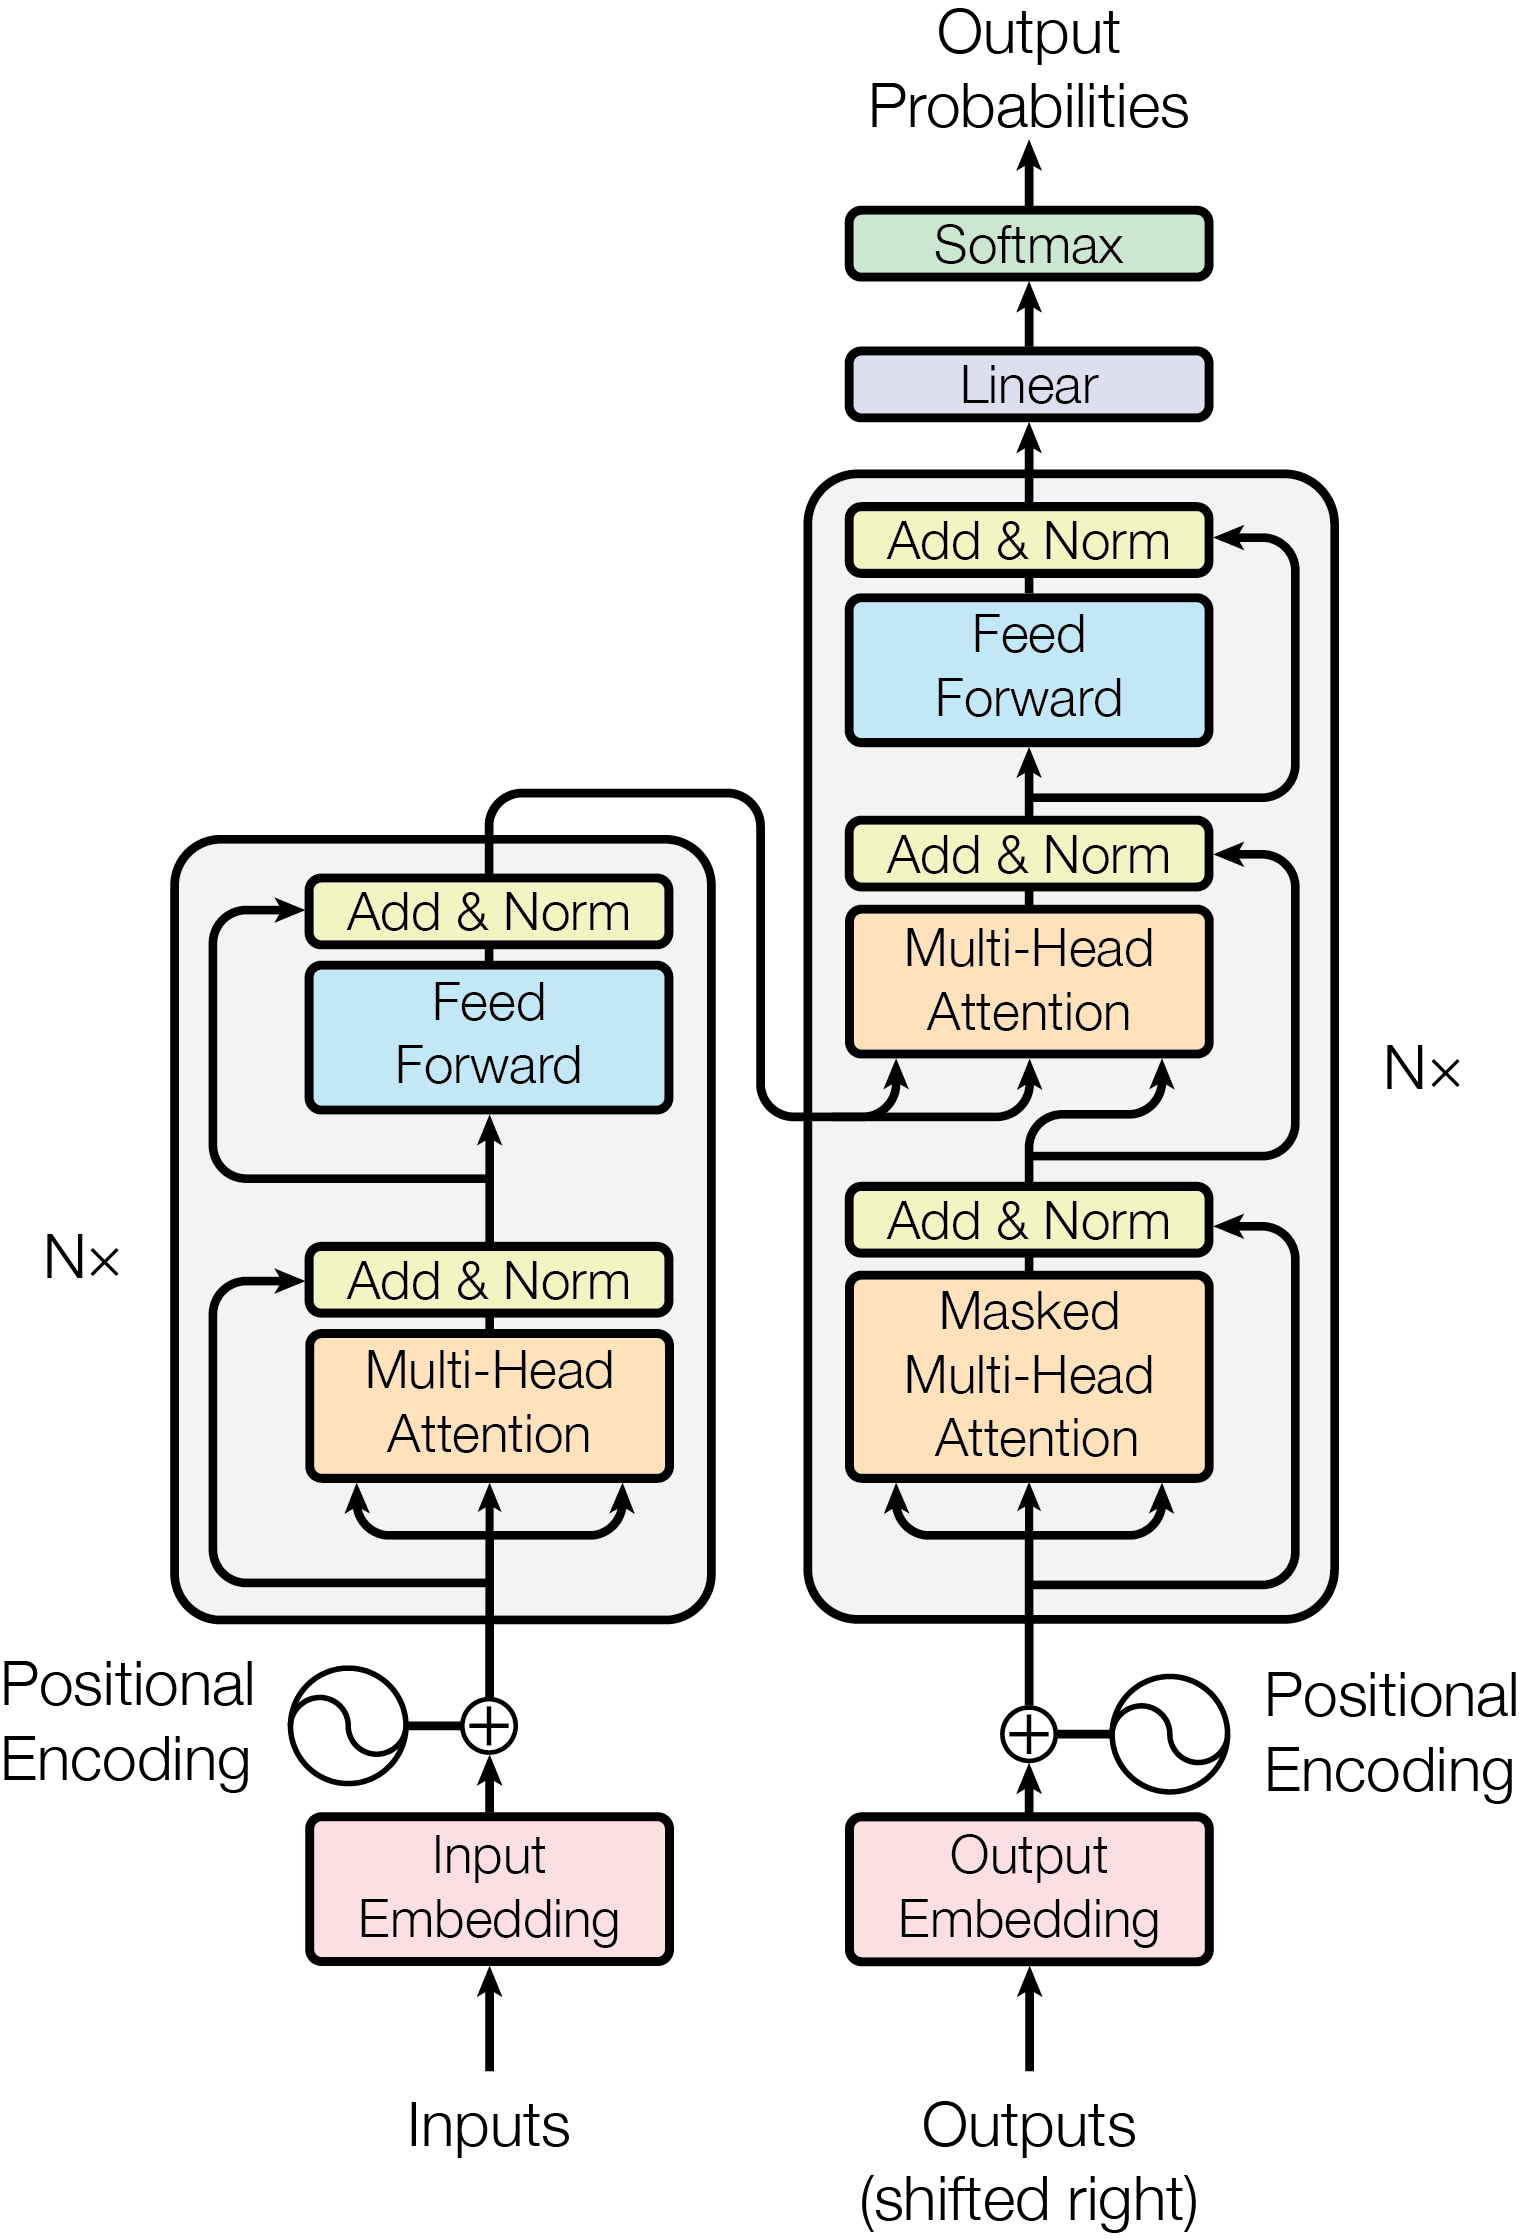
\includegraphics[width=0.6\textwidth]{transformer.png}
    \caption{The transformer architecture \citep[figure taken from][]{vaswani2017attention}.}
    \label{fig:transformer_architecture}
\end{figure}

\noindent The transformer~\citep{vaswani2017attention} is an architecture which
maps an input sequence to an output sequence through many layers of
\textbf{multi-head attention} mechanisms, yielding a dynamic,
context-dependent strategy for propagating information within and
across sentences. It contrasts with previous seq2seq models for neural machine translation (NMT), which
usually rely either on gated recurrent operations~\citep[often
    LSTMs:][]{bahdanau2014neural,luong2015effective} or static
convolutions~\citep{convseq}. A diagram of this architecture is
shown in \figref{fig:transformer_architecture}.

Attention mechanisms compute, for each query, a weighted
representation of the items. The particular attention mechanism used
in \citet{vaswani2017attention} is called \emph{scaled dot-product
    attention}.

\begin{definition}[attention mechanisms and scaled dot-product attention]
    Attention mechanisms are a possible differentiable building block
    of a neural network, mainly used in sequence modeling. For each
    item in the sequence, the attention mechanism computes a weighted
    representation of all the other items in said sequence or a given
    context sequence. Given the current item, it can often be
    interpreted as showing each item's importance in the context. A
    scaled dot-product attention mechanism is a particular type of
    attention mechanism:
    %
    \begin{equation}
        \att(\bm{Q}, \bm{K}, \bm{V}) = \amap
        \left(\frac{\bm{Q}\bm{K}^\tr}{\sqrt{d}}\right) \bm{V},
        \label{eq:att_scaled_dot}
    \end{equation}
    %
    where, given $n$ query contexts and $m$ sequence items under
    consideration, $\bm{Q} \in \reals^{n \times d}$ contains
    representations of the queries, $\bm{K}, \bm{V} \in \reals^{m
            \times d}$ are the \emph{keys} and \emph{values} of the items
    attended over, and $d$ is the dimensionality of these
    representations. The $\amap$ mapping normalizes row-wise using a mapping function like
    \textbf{softmax}, that is, $\amap(\bm{Z})_{ij} = \softmax(\bm{z}_i)_j$.
    In words, the \emph{keys} compute a relevance score between each item
    and query. Then, $\amap$ normalizes these attention weights, and
    these will weight the \emph{values} of each item at each query
    context.
\end{definition}

However, for complex tasks, different parts of a sequence may be
relevant in different ways, motivating \emph{multi-head attention} in
transformers. Multi-head attention is simply the application of
\eqnref{eq:att_scaled_dot} in parallel $H$ times, each with a
different learned linear transformation that allows specialization,
%
\begin{equation}\label{eq:head}%
    \ath_i(\bm{Q}\!,\!\bm{K}\!,\!\bm{V})\!=\!\att(\bm{QW}_i^Q\!\!,\bm{KW}_i^K\!\!,\bm{VW}_i^V\!).
\end{equation}

In the transformer, there are three separate multi-head attention mechanisms for
distinct purposes:
%
\begin{itemize}
    \item \textbf{Encoder self-attention:} builds rich, layered representations of
          each input word by attending to the entire input sentence;
    \item \textbf{Context attention:} selects
          a representative weighted average of the encodings of the input words at each
          time step of the decoder;
    \item \textbf{Decoder self-attention:} attends over the partial output sentence
          fragment produced so far.
\end{itemize}
%
Together, these mechanisms enable the contextualized flow of information between
the input sentence and the sequential decoder.

\subsection{Large Pre-trained Language Models}
\label{sec:pretrained-bg}

\noindent A recently attractive way to obtain high-performing models in NLP is
to use a pre-trained language model. These are models with many
parameters, trained on millions of sentences gathered from
the web, using many computational resources in the training process.
Many such models are publicly released and are
available for the research and industry community to use. Typically,
practitioners download an already optimized model from the web and
train it further by \textit{finetuning} it, that is, taking an
already trained model's parameters and optimizing them on a new
dataset, usually using a lower learning rate, such that the new
optimum does not veer too far from the original optimum.

Many different models have been released in the last few years, such
as ELMo~\citep{peters2018deep}, OpenAI GPT
series~\citep{radford2018improving, brown2020language},
BERT~\citep{devlin2018bert}, and
T5~\citep{raffel2020Exploringlimitstransfer}. Of particular interest
in this thesis is BERT since it is the model used in
\chapref{chap:ape}.

BERT, at its core, is a transformer model, as described in
\secref{sec:transformer_bg}. However, it is only made out of the
encoder building block and thus does not have language modeling
capabilities in its \textit{vanilla} form. As is the case with other
similar models, BERT was trained on an enormous corpus of sentences
in monolingual English and in multilingual datasets of 100+
languages. BERT's masked language modeling objective (MLM) has proven
to be a powerful mechanism to learn transferrable contextual encoder
representations of tokens and sentences. Many works have analyzed
the BERT model and have developed variants for it. Its study has even
been referred as ``BERTology''~\citep{rogers2020PrimerBERTologyWhat}.
